\documentclass[../../../../main.tex]{subfiles}
\begin{document}

\begin{flushright}
\footnotesize\textit{【自動文字起こし・要確認】}
\end{flushright}

[解]\\
$BC : \frac{x}{b} + \frac{y}{c} = 1$\\
$l : b(x-b) - cy = 0$\\
$m : bx - c(y-c) = 0$\\
だから、$P(bX, cY)$ とおくと ($X+Y=1$)\\
$Q\left(bX, \frac{b^2}{c}(X-1)\right), R\left(\frac{c^2}{b}(Y-1), cY\right)$\\
だから $X+Y=1$ から
\[ \overrightarrow{AQ} = \begin{pmatrix} bX \\ -\frac{b^2}{c}Y \end{pmatrix}, \overrightarrow{AR} = \begin{pmatrix} -\frac{c^2}{b}X \\ cY \end{pmatrix} \]
となり、$\overrightarrow{AQ} \parallel \overrightarrow{AR}$ だから、$Q, R, A$ は一直線上にある (図)\\

\begin{tikzpicture}
\draw[->] (-1,0) -- (4,0) node[right] {$x$};
\draw[->] (0,-1) -- (0,3) node[above] {$y$};
\coordinate (A) at (0,0);
\coordinate (B) at (3,0);
\coordinate (C) at (0,2);
\coordinate (P) at (1.5,1);
\coordinate (Q) at (1.5,-1.125);
\coordinate (R) at (-2,1);

\draw (B) -- (C);
\node[below left] at (A) {A};
\node[below] at (B) {B};
\node[left] at (C) {C};
\node[above right] at (P) {P};

\draw[dashed] (P) -- (Q);
\draw[dashed] (P) -- (R);
\node[below] at (Q) {Q};
\node[left] at (R) {R};
\draw (B) -- (1.5, -1.125) node[midway, right] {$l$};
\draw (C) -- (-2, 1) node[midway, above] {$m$};
\end{tikzpicture}

(2) 図のように定めると、題意の時
\[ \frac{1}{2} (\alpha + \gamma) \cdot h = 2 \cdot \frac{1}{2} \beta h \]
\[ \alpha + \gamma = 2\beta \quad \cdots \text{①} \]
である。

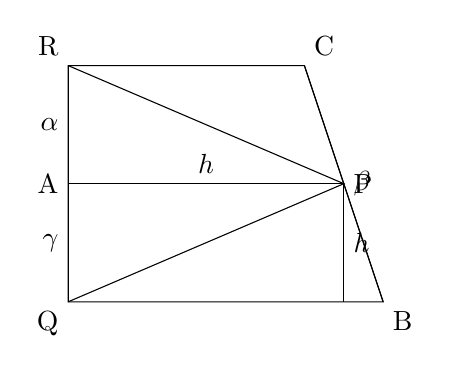
\begin{tikzpicture}
\coordinate (R) at (0,3);
\coordinate (C) at (3,3);
\coordinate (A) at (0,1.5);
\coordinate (Q) at (0,0);
\coordinate (B) at (4,0);
\coordinate (P) at (3.5, 1.5);

\draw (R) -- (C) -- (B) -- (Q) -- cycle;
\draw (R) -- (P) -- (Q);
\draw (C) -- (P) -- (B);
\draw (A) -- (P);

\node[above left] at (R) {R};
\node[above right] at (C) {C};
\node[left] at (A) {A};
\node[below left] at (Q) {Q};
\node[below right] at (B) {B};
\node[right] at (P) {P};

\node[left] at (0, 2.25) {$\alpha$};
\node[left] at (0, 0.75) {$\gamma$};
\node[right] at (3.5, 1.5) {$\beta$};

\draw (P) -- (0, 1.5) node[midway, above] {$h$};
\draw (P) -- (3.5, 0) node[midway, right] {$h$};
\end{tikzpicture}

\begin{itemize}
\item[$1^\circ$] $\text{RQ} \not\parallel \text{BC}$ の時\\
①なら AはRQの中点であり（ $\because$ \\
$|AQ|^2 = |AR|^2$\\
$\iff b^2 X^2 + \frac{b^4}{c^2} Y^2 = c^2 Y^2 + \frac{c^4}{b^2} X^2$\\
$\iff \frac{b^4 - c^4}{c^2} Y^2 = \frac{c^4 - b^4}{b^2} X^2$\\
$\iff \frac{Y^2}{c^2} = -\frac{X^2}{b^2} \quad (\because b \neq c)$\\
となり、$b, c, X, Y \in \mathbb{R}$, $X+Y=1$ に矛盾。よってこの時①のようにはならない

\item[$2^\circ$] $\text{RQ} \parallel \text{BC}$ の時\\
AはRQ上の任意の点で①をみたす（ $\because X = \frac{b^2}{b^2+c^2} \quad (0 < \frac{b^2}{b^2+c^2} < 1)$ となれば、$\overrightarrow{AQ} \parallel \overrightarrow{BC}$ となって適する）\\
以上から①のようになるのは $\text{RQ} \parallel \text{BC}$ の時で、この時、題意から\\
$\square \text{BCRQ} \text{は長方形}$\\
である。
\end{itemize}

\end{document}
